\documentclass{article}

\usepackage[margin=1.5in]{geometry}
\usepackage{graphicx}
\usepackage{xfrac}
\usepackage{amsmath}
\usepackage{amssymb}
\usepackage[linesnumbered,lined,ruled]{algorithm2e}
\usepackage[skip=2pt,labelfont=bf]{caption}

\newtheorem{mydef}{Definition}
\let\emph\textbf

\title{A brief survey on two exact algorithms for the knapsack problem}
\author{Marcos Daniel Baroni}

%%%%%%%%%%%%%%%%%%%%%%%%%%%%%%%%%%%%%%%%%%%%%%%%%%%%%%%%%%%%%%%%%%%%%%%%%%%%%%%%
% Objetivo: Apresentar resumidamente os resultados dos testes que fiz sobre
%  tempo esperado do backtrack para o KP;
%  - Comentar sobre artigos:
%    - [1] "On the avrg diff between the solutions to LP and IP KPs"; (comentário, qualidade de solução)
%    - [2] "On finding the Exact Solution of 0-1 KP";
%    - [3] "Random KP in Expected PTime";
%  (- Lembrar que KP:
%     1. é NP-Completo para coeficientes ilimitados;
%     2. admite FPTAS em número de itens;)
%  - Apresentar o algoritmo backtrack para o KP;
%  - Apresentar algoritmo de Programação Dinâmica 
%%%%%%%%%%%%%%%%%%%%%%%%%%%%%%%%%%%%%%%%%%%%%%%%%%%%%%%%%%%%%%%%%%%%%%%%%%%%%%%%

%%%%%%%%%%%%%%%%%%%%%%%%%%%%%%%%%%%%%%%%%%%%%%%%%%%%%%%%%%%%%%%%%%%%%%%%%%%%%%%%
% Seção 1: O KP (FPTAS, NP-Completeness, polinomial expectance, )
%    Definição do problema/relaxação LP;
%    Algoritmo Greedy para a relaxação e diferença entre soluções [1];
% Seção 2: O algoritmo de backtrack ()
%    Apresentação 
% Seção 3: O algoritmo de Prog. Dinamica de Beier
% Seção 4: Resultados
%    *Curva1: Nós abertos até encontrar a melhor (polinomial);
%    *Curva2: Nós abertos até provar a melhor (conjectura: 1.8^(x-3) );
%    [2] Citar probabilidade de encontrar a melhor solução;
%%%%%%%%%%%%%%%%%%%%%%%%%%%%%%%%%%%%%%%%%%%%%%%%%%%%%%%%%%%%%%%%%%%%%%%%%%%%%%%%

\begin{document}

\maketitle

This brief study was inspired by a comment about backtracking approach for knapsack problem
by Lueker in \cite{lueker1982average} 
saying:

\vspace*{10pt}
\begin{minipage}{5in}
``{\it When applied to randomly generated data, this approach, which always yields the
exact optimum, seems to run very rapidly even for large values of $N$; in fact,
it seems possible that its expected time is polynomial in $N$. A proof of this
would be very interesting, but probably difficult}''.
\end{minipage}
\vspace*{10pt}

The knapsack problem is briefly introduced in Section~\ref{sec:kp}.
The backtrack algorithm for the knapsack problem and some experimental results
is presented in Section~\ref{sec:backtrack}.
A sparse dynamic programming approach for the knapsack problem is presented in
Section~\ref{sec:dp}.

\section{The knapsack problem}
\label{sec:kp}

In this report we consider the $0/1$ knapsack problem which can be defined as follows:
given $n$ positive weights $w_i$, $n$ positive profits $p_i$ and a positive
number $b$ which is the knapsack capacity, this problem calls for choosing a
subset $s \in [n]$ such that
\begin{displaymath}
  max \sum_{i \in s} p_i x_i \qquad \text{subject to} \qquad
  \sum_{i \in s} w_i x_i \leqslant b
\end{displaymath}
The $x$ constitutes a $0/1$ valued vector.
To facilitate greedy procedures we can consider the items is sorted in
nondecreasing order of {\it profit density}:
  ${p_1 \over w_1} \geqslant {p_2 \over w_2} \geqslant \ldots \geqslant {p_n \over w_n}$.

\section{The backtracking approach}
\label{sec:backtrack}
The backtrack procedure is a general technique used to solve combinatorial
problems dealing with search for a set of solutions or an optimal
solution satisfying some constraint.

In order to apply the backtrack method the desired solution must (a) be
expressible as an $n$-tuple $(x_1, x_2, \ldots, x_n)$ where $x_i$ are chosen
from some finite set $S_i$ and (b) shares a property $P_n(x_1, \ldots, x_n)$
such that $P_{k+1}(x_1, \ldots, x_k, x_{k+1})$ implies $P_{k}(x_1, \ldots, x_k)$
for $0 \leqslant k \leqslant n$.

The backtrack procedure consists of enumerating all solutions $(x_1, \ldots, x_n)$
to the original problem by computing all partial solutions $(x_1, \ldots, x_k)$
that satisfy $P_k$.
If a partial solution $(x_1, \ldots, x_k)$ does not satisfying $P_k$; hence by induction,
no extended sequence $(x_1, \ldots, x_k, \ldots, x_n)$ can satisfy $P_n$.

In the case of knapsack problem, each partial solution $(x_1, \ldots, x_k)$ can be
viewed as a subproblem whose variables $x_1, \ldots, x_k$ are fixed while $x_{k+1}, \ldots,
x_n$ are free.
For each subproblem a relaxed version can be derived
replacing the integrality contraints of the free variables
by the linear relaxation constraint $x_i \in [0, 1]$.
This relaxation is called {\it linear relaxation}.
The linear relaxation can be used to prune its respective partial solution:
whenever its optimal value is not better than the best optimal solution found so far,
the respective partial solution is pruned and the algorithm backtracks.

The solution for linear relaxation of a given partial solution is given by
the greedy algorithm (Algorithm~\ref{alg:greedy}).

\begin{algorithm}[H]
 \SetKwInOut{Input}{Input}
 \SetKwInOut{Output}{Output}
 \SetKwComment{Comment}{}{}
 \Input{ a partial solution $(x_1, \ldots, x_k)$ }
 \Output{ the LP upper bound $p_{lp}$}
 $b_{lp} \leftarrow b$\;
 $p_{lp} \leftarrow 0$\;
 \For(\tcc*[f]{compute current profit and weight}){$i \leftarrow 1$ \KwTo $k$}{
 	$b_{lp} \leftarrow b_{lp} + x_i \cdot w_i$;
 	$p_{lp} \leftarrow p_{lp} + x_i \cdot p_i$\;
 }
 \While(\tcc*[f]{greedily filling knapsack}){$b_{left} \geqslant w_i$}{
 	$b_{lp} \leftarrow b_{lp} + w_i$;
 	$p_{lp} \leftarrow p_{lp} + p_i$;
	$i \leftarrow i+1$\;
 }
 $p_{lp} \leftarrow p_{lp} + p_i.\frac{b_{lp}}{w_i}$\tcc*[f]{fitting the split item}
 \caption{Computes profit of LP-relaxation of a partial solution}
 \label{alg:greedy}
\end{algorithm}

Figure~\ref{fig:experiment} shows experimental results on the number of partial
solutions computed by the backtrack algorithm.
The continuous line is the average number over 1000 random instances,
the dotted line is the total number of possible solutions and
the dashed line is the conjectured curve for the observed experimental result;
(a) shows the number of computed solutions to find the optimal solution and
(b) shows the number of computed solutions to prove its optimality.

\section{The Nemhauser-Ullmann algorithm}
\label{sec:dp}
%A brute force method to solve the knapsack problem is to enumerate all possible subsets over the $n$ items.
In order to reduce the search space of a knapsack problem instance, a domination
concept can be used which is usually attributed to Weingartner and Ness~\cite{weingartner1967methods}.
\begin{mydef}[Domination]
A subset $S \in [n]$ with weight $w(S) = \sum_{i \in S} w_i$  and profit $p(S) = \sum_{i \in S} p_i$
\emph{dominates} another subset $T \subseteq [n]$ if $w(S) \leqslant w(T)$ and $p(S) \geqslant p(T)$.
\end{mydef}

For simplicity assume that no two subsets have the same profit.
Then no subset dominated by another subset can be an optimal solution to the knapsack problem, regardless of the specified knapsack capacity.
Consequently, it suffices to consider those sets that are not dominated by any other set.

Using this concept Nemhauser and Ullmann~\cite{nemhauser1969discrete} introduced an elegant
algorithm (Algorithm~\ref{alg:nu}) computing a list of all dominating sets in an iterative manner.

\begin{algorithm}[H]
 \SetKwInOut{Input}{Input}
 \SetKwInOut{Output}{Output}
 \Input{a KP instance}
 \Output{list $S(n)$ of all dominating sets}
 $S(0) \leftarrow \emptyset $\;
 \For{$i\leftarrow 1$ \KwTo $n$}{
   $S'(i) \leftarrow S(i-1)\; \cup \big\{ s \cup \{i\} \,\big|\, s \in S(i-1)\big\}$\;
   %$S(i) \leftarrow \big\{ s \,\big|\, s \in S'(i), dominates\big(s, S'(i)\big) \big\}$\;
   $S(i) \leftarrow \big\{ s \in S'(i) \,\big|\, \mathsf{dominates}\big(s, S'(i)\big) \big\}$\;
   %$S(i) \leftarrow \emptyset $\;
   %\ForEach{$ s \in S'(i)$}{
   %   \If{$ dominates\big(s, S'(i)\big)$}{
   %      $S(i) \leftarrow S(i) \cup \{s\}$\;
   %  }
   %}
 }
 \caption{The Nemhauser-Ullmann Algorithm}
 \label{alg:nu}
\end{algorithm}

%Let $S(i)$ be the sequence of dominating subsets over the items $1, \ldots, i$.
%Given $S(i-1)$, the sequence $S(i)$ can be computed as follows:
%Now we compute $S(i)$ by selecting just the dominating sets in $S'(i)$ (line 4).
This algorithm can be viewed as a sparse dynamic programming approach which
at each iteration duplicates all subsets in $S(i-1)$ and then adds item $i$
to each of the duplicated subsets (line 3).
The $\mathsf{dominates}$ procedure checks if subset $s$ dominates all others subsets in $S'(i)$.
The dominated subsets are then {\it filtered} (line 4).
The result is the ordered sequence $S(n)$ of dominating subsets over the items $1, \ldots, n$.

Figure~\ref{fig:pareto} graphically represents profits and weights for
dominating sets of (a) an intermediate solution $S(i)$,
(b) its next solution $S(i+1)$ and (c) an optimal solution for a small random instance.

If we denote $q(i)$ the upper bound on the number of dominating sets over items in
$1, \ldots, i$, at each iteration the algorithm computes $S(i)$ over $S(i-1)$ in $O\big(q(i)\big)$ time.
The total running time of the algorithm is then $O\big(n \cdot q(n)\big)$.
Now the challenge in the analysis is to estimate the number of dominating sets.

Beier and V{\"o}cking~\cite{beier2003random} addressed this analysis considering
sets of items with adversary weights and randomly drawn profits.
They could deduce that for the uniform distribution, for example, the expected
number of dominating sets is $E[q] = O(n^3)$ leading to an expected running
time of $O(n^4)$.

\begin{figure}[h]
  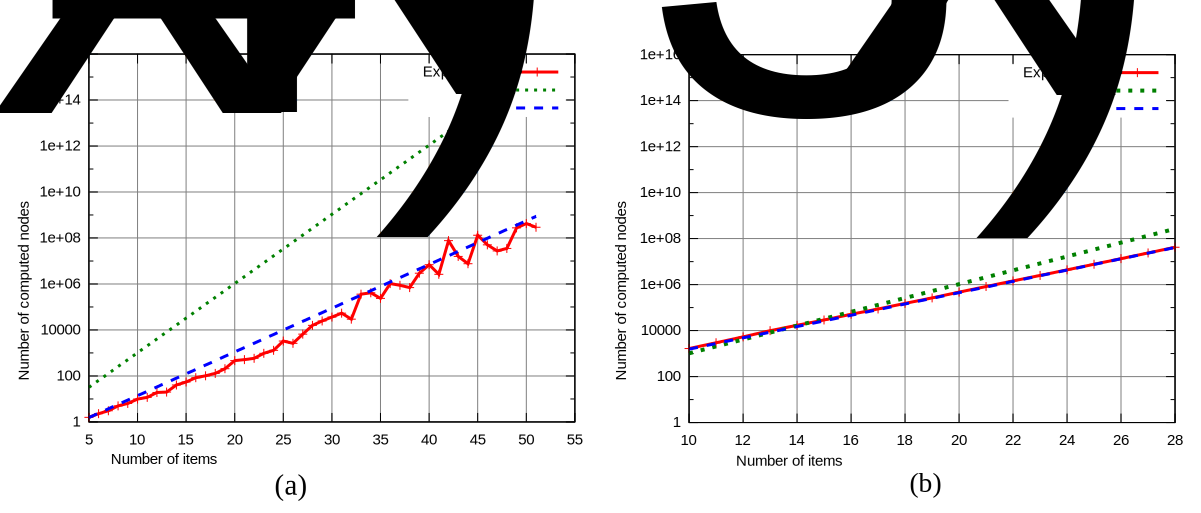
\includegraphics[width=\textwidth]{find-proof}
  \caption{Number of computed nodes (partial solutions) (a) to find the optimal solution
  and (b) to prove its optimality.}
  \label{fig:experiment}
\end{figure}

\begin{figure}[h]
  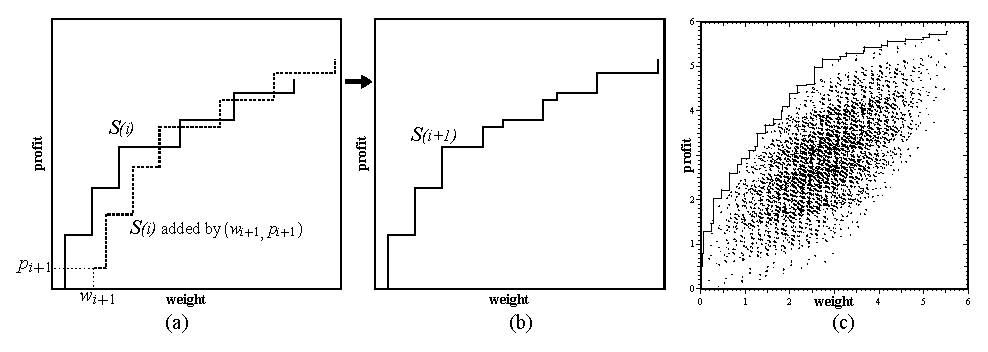
\includegraphics[width=\textwidth]{pareto}
  \caption{Graphical representation of dominating sets for
  (a) an intermediate solution $S(i)$, (b) its next solution $S(i+1)$. and
  (c) an optimal solution for a small random instance.}
  \label{fig:pareto}
\end{figure}

\newpage 

\bibliographystyle{abbrv}
\bibliography{../../refs}

\end{document}

